\chapter{Product Design}
\section{Product Functions}
When complete the device driver should be able to fully facilitate a communication between the host and the controller. This means that all the features supported by BlueNRG must function depending on how the user is willing to use them through the host. To learn more about the functionality offered by BlueNRG, one needs to go through BLE, what is is and what it has to offer. The subsequent sections of the report present a detailed case of the same.
\section{Bluetooth Low Energy}
Bluetooth low energy (\textbf{BLE}, marketed as \textbf{Bluetooth Smart}) is a wireless personal area network technology designed and marketed by the \textbf{Bluetooth Special Interest Group aimed} at novel applications in the healthcare, fitness, beacons, security, and home entertainment industries. \\
It is part of the Bluetooth \textbf{4.0 specification}. It aims at being a low energy, low cost, low bandwidth, low power and low complexity extensible framework for exchanging data pertaining to various applications fields. 
\subsection{Device Configuration}
\begin{itemize}
	\item \textbf{Single mode Devices} (Bluetooth smart): These devices are compatible to BLE only. Examples are typically small devices like Heart monitors, sensors, other low-power consuming application hardware.
	\item \textbf{Dual mode Device} (Bluetooth smart ready): These device are compatible to both BLE and traditional BR/EDR. Example of this kind of devices are PCs, Tablets and smartphones i.e. devices with larger battery or power consumption.
\end{itemize}
\begin{figure}[ht]
	\centering
	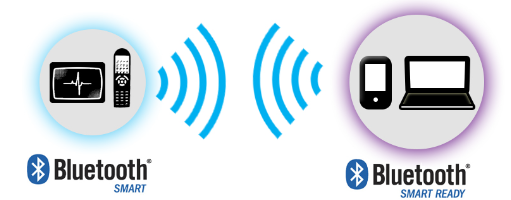
\includegraphics[scale=0.5]{images/device_configuration.png}
	\caption{BLE Device Configuration}
\end{figure}
\subsection{Limitations}
Bluetooth Low Energy has been designed with some specific fundamentals that happen to serve in a lot of application fields. But this means that it is not apt other kind of applications. Most of its limitations are due to the following two fundamental fact
\begin{enumerate}
	\item The maximum theoretical throughput is \textbf{1Mbps} which is reduces by several factors to only \textbf{5-10KBps} in most cases
	\item The operating range is generally \textbf{2-5 meters}. This can be extended to \textbf{30 meters} or so but that will of course demand higher strain on the battery life of the devices. This is the defining thing about the BLE technology that the devices are mostly passive in nature and hence it becomes very important for them to have large battery life. In some cases it is seen that the device’s battery can actually outlast other hardware in the device itself
\end{enumerate}
\subsection{Bluetooth Low Energy Network Topologies}
Network topology defines the way in which different devices (under different roles) interact with one another to exchange data through BLE. These topologies are defined within the specification and are maintained under the guidelines established by Generic Access Profile (GAP).\\
Following three topologies are found in BLE:
\begin{enumerate}
	\item Broadcasting and Observing
	\item Connection oriented
	\item Mixed topology
\end{enumerate}
Let’s take a look at them individually.
\subsubsection{Broadcasting}
A device (broadcaster) sends out advertising packets (after fixed intervals) to any device that is willing to scan this packet and extract data from it. The observing device also scans for any advertising packets in its range after a fixed interval. When these two intervals (advertising and scanning) overlap, then the devices are able to exchange data among themselves.\\
Data broadcasting by a device can be picked up any observer. Observer can choose to acknowledge this reception or not.\\
Advertising packets contains data up to \textbf{31 bytes}. This can be extended by another packet if requested by any observer using the \textbf{scan request packet}.
\begin{figure}[ht]
	\centering
	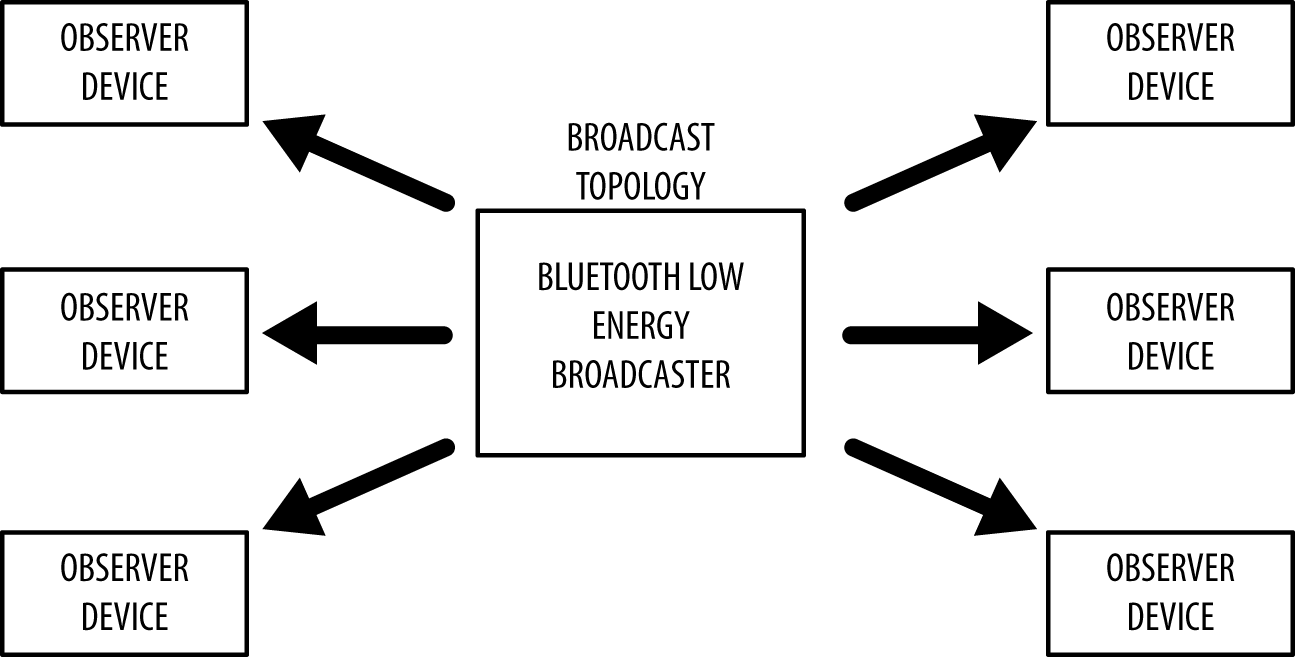
\includegraphics[width=3.5in, height=3in]{images/broadcast_topology.png}
	\caption{Broadcasting and Observing Topology}
\end{figure}
\subsubsection{Connections}
A connection is a permanent, periodical data exchange of packets between two devices. It is therefore inherently private (the data is sent to and received by only the two peers involved in a connection, and no other device unless it is indiscriminately sniffing).\\
This topology is useful when one wants to communicate in both directions and the data to be communicated cannot be accommodated in two advertising packets.\\
Connections involve two separate roles: \textbf{Master} (scans for any device advertising to be in a connection) and \textbf{Slave} (advertises at intervals to be a part of an exclusive connection and accepts a connection request from a master to establish the connection).
\begin{figure}[ht]
	\centering
	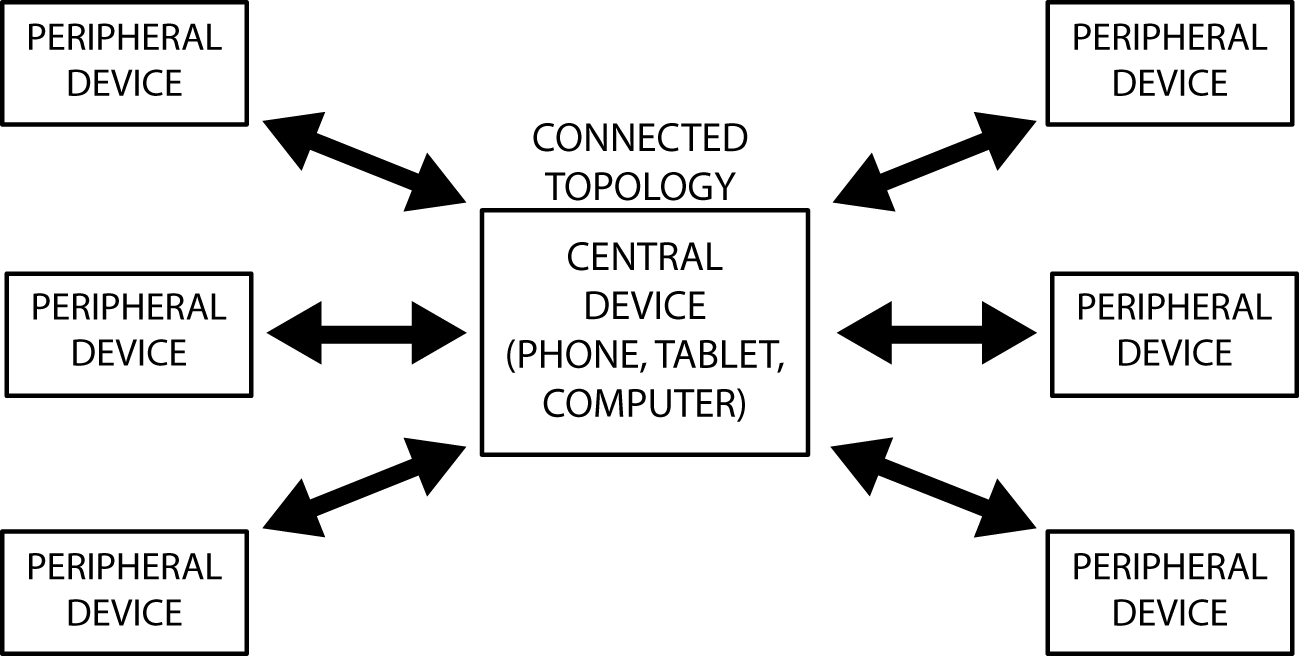
\includegraphics[width=3.5in, height=3in]{images/connected_topology.png}
	\caption{Connection Topology}
\end{figure}
\subsubsection{Mixed Topology}
The previous two topologies can be mixed freely in a wider BLE network, as shown in the figure below. A BR/EDR/LE capable device can bridge together BLE and BR/EDR connections, and the number of combinations and participants on the network is constrained only by the limitations of the radios and protocol stacks of each device taking part in it.
\begin{figure}[ht]
	\centering
	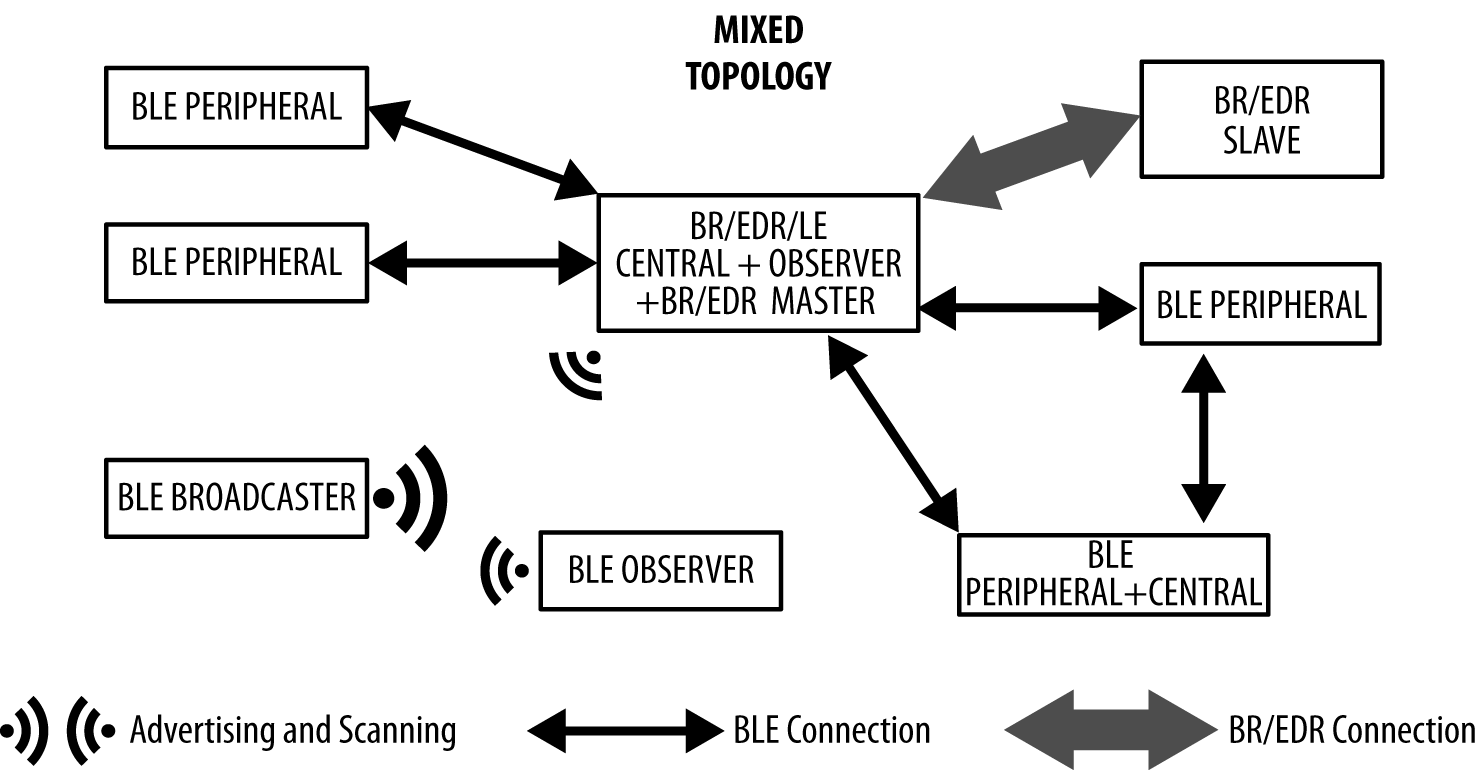
\includegraphics[width=3.5in, height=3in]{images/mixed_topology.png}
	\caption{Mixed Topology}
\end{figure}
\subsection{BLE Architecture}
The complete BLE protocol stack is divided into layers that work and communicate in succession to achieve the desired operation.\\
These layers are:
\begin{enumerate}
	\item \textbf{Application} (The upper layer containing most of the application logic, User interface, etc)
	\item \textbf{Host} (Contains all the upper layer protocols like GAP, GATT, L2CAP, etc.)
	\item \textbf{Controller} (Contains all the lower layer protocols from the Link Layer and the Physical Layer.)
\end{enumerate}
The host layer and the controller layer communicate with each other using the \textbf{Host Controller Interface} (HCI). This allows great flexibility in having the host and controller on different chips and having different manufactures.
\begin{figure}[ht]
	\centering
	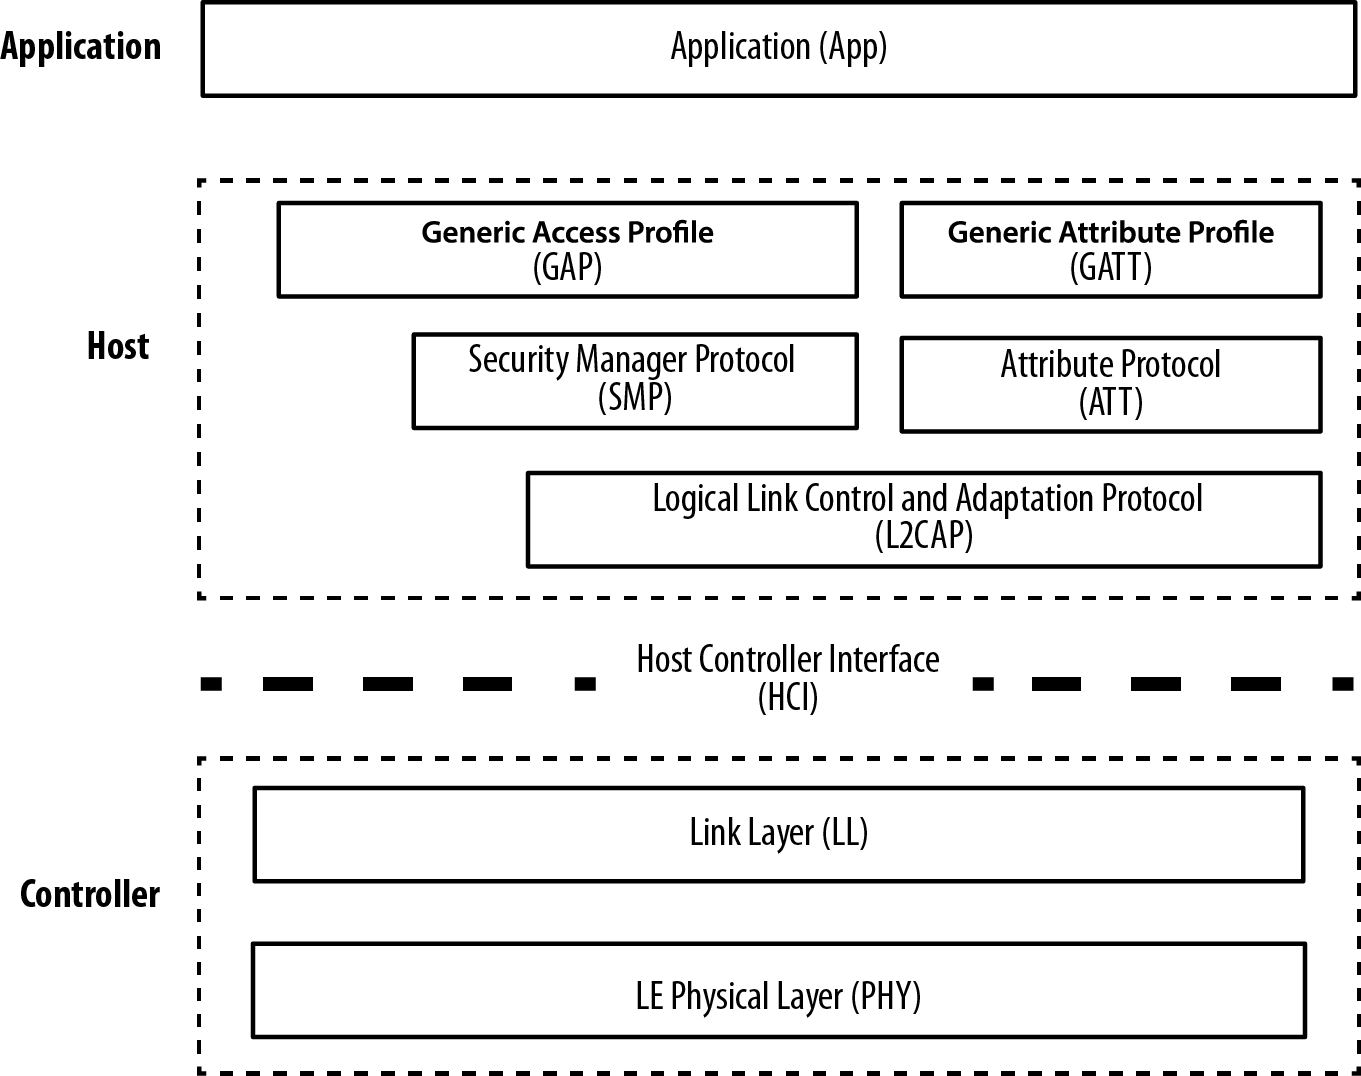
\includegraphics[scale=0.2]{images/ble_architecture.png}
	\caption{BLE Architecture}
\end{figure}
\subsection{Classification of devices based on Chip Count}
Like devices can be classified on the basis of different compatibility modes, they can also be classified on the basis of the chip configuration of the various layers of BLE.
\begin{enumerate}
	\item \textbf{SoC (System on Chip)}: A single IC runs the application, the host, and the controller.
	\item \textbf{Dual IC over HCI}: One IC runs the application and the host and communicated using HCI with a second IC running the controller.
	\item \textbf{Dual IC with connectivity device}: One IC runs the application and communicates using a proprietary protocol with a second IC running both the host and the controller. BlueNRG uses this chip configuration.
\end{enumerate}
\begin{figure}[ht]
	\centering
	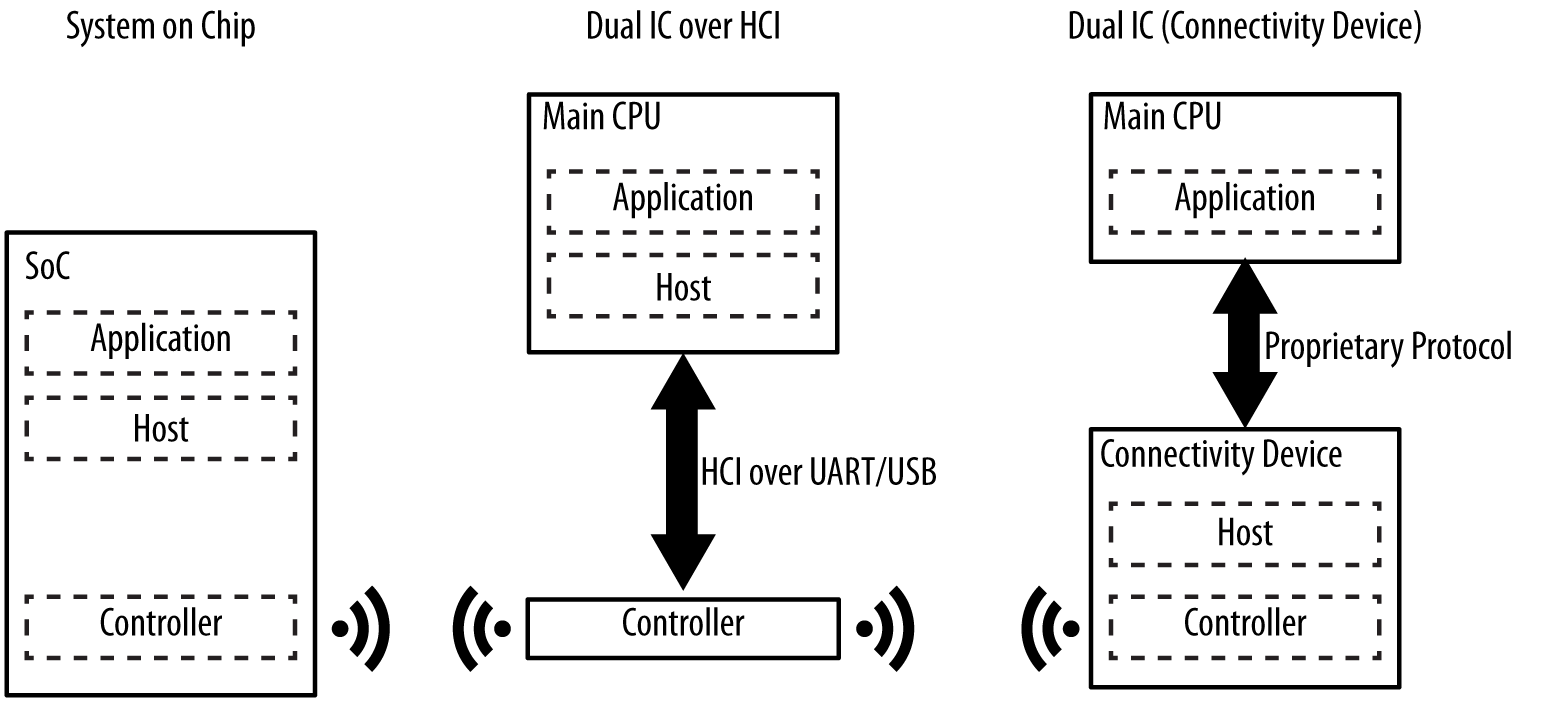
\includegraphics[scale=0.2]{images/chip_count.png}
	\caption{Classification based on chip count}
\end{figure}
\subsection{The Protocol Stack}
The whole BLE protocol stack is divided into layers. This makes it easier to study and apply the protocol because otherwise the protocol is not as plainly vertical as some other protocols are like the TCP/IP. The layers are:
\begin{enumerate}
	\item \textbf{The Controller Layer}
	\item \textbf{The Host Layer}
	\item \textbf{The Application Layer}
\end{enumerate}
\subsection{The Controller Layer}
This contains the lower layer of protocol like:
\subsubsection{The Physical Layer}
This layer is responsible for the analog transmission and AC-DC conversions. Bluetooth utilized the 2.4 GHz ISM bandwidth with 40 2MHz channels. Out of these 40 channels, 37 are for data transfer that is to occur once the connection has been established between participating devices. The other 3 channels are for broadcasting, observing and advertising.\\
The specification uses the frequency hopping spread spectrum to prevent overlapping interference of channels. This hopping takes place simultaneously and is based on the following equation:\\
Channel = (CurrentChannel + Hop) mod 37\\
The modulus of 37 obviously is there to round of the channel number to stay between 0 and 36 i.e. the available data channels for connections. The value of hop is known only to the connected devices and this hence enables them to hop to the same channels at the same time and no one else will be able to interfere between them.
The Gaussian Frequency Shift Keying (\textbf{GFSK}) is used to encode the bit stream over the air.
\begin{figure}[ht]
	\centering
	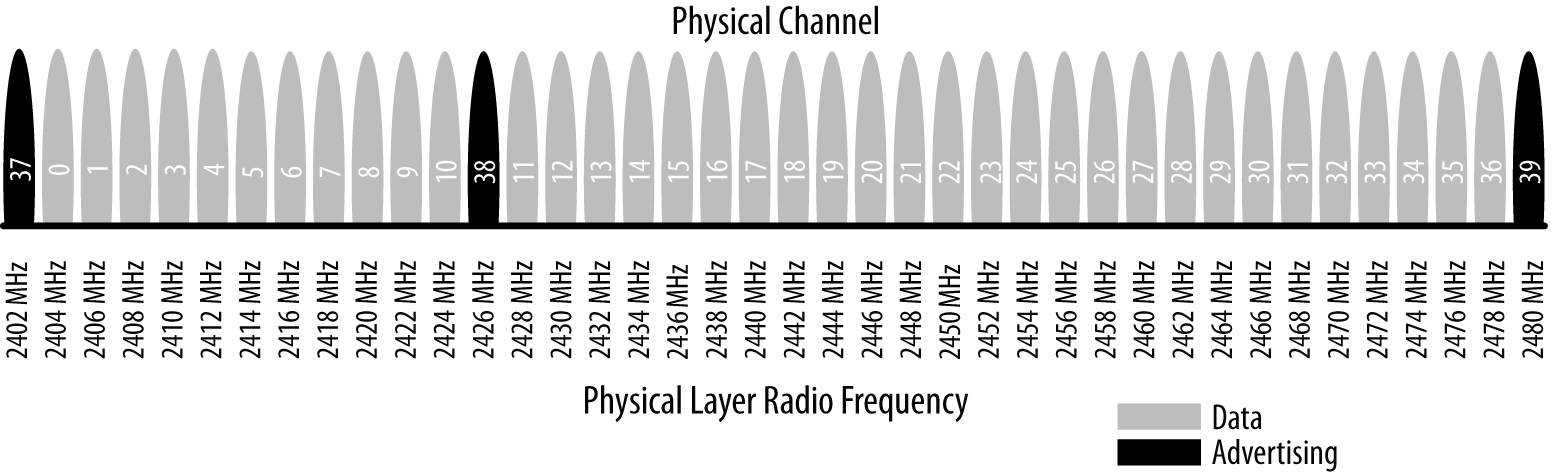
\includegraphics[scale=0.3]{images/physical_channel.png}
	\caption{The 40 physical channels}
\end{figure}
\subsubsection{Link Layer}
The Link Layer is responsible for complying with all of the timing requirements defined by the specifications and managing device connections. It also performs CRC, Data whitening, Random number generations, AES encryption, etc.\\
The Link Layer defines the following roles:
\begin{enumerate}
	\item \textbf {Advertiser}: A device sending advertising packets.
	\item \textbf {Scanner}: A device scanning for advertising packets.
	\item \textbf {Master}: A device that initiates a connection and manages it later.
	\item \textbf {Slave}: A device that accepts a connection request and follows the master’s timing.
\end{enumerate}
These roles can be logically grouped into two pairs: advertiser and scanner (when not in an activie connection) and master and slave (when in connection).
\paragraph{Link Layer Bluetooth Device Addresse}
This is the fundamental identifier of a Bluetooth device, similar to an Ethernet Media Access Control (MAC) address. It is \textbf{ 6 bytes} long. \\
There are two types of device addresses, and on or both can be set on a particular device:
\begin{enumerate}
	\item \textbf{Public Device Address}: This is factory-programmed device address. Registered with \textbf{IEEE} registration authority and never changes during the lifetime of the device.
	\item \textbf{Random Device Address}: This address can either be preprogrammed on the device or dynamically generate at runtime. It can be used to achieve privacy when in a connection.
\end{enumerate}
\paragraph{Link Layer Advertising and Scanning}
The advertising packets are used to either broadcast data for applications or to discover slaves and to connect to them. The advertising of packets is done after certain intervals and if during this interval some device is scanning then that device will be able to receive the advertising packet.\\
The specification defines two basic types of \textbf{scanning procedures}:
\begin{enumerate}
	\item \textbf{Passive Scanning}: The scanner simply listens for advertising packets, and the advertiser is never aware of the fact that one or more packets were actually received by a scanner.
	\item \textbf{Active Scanning}: The scanner issues s Scan Request packet after receiving an advertising packet. The advertiser receives it and responds with a Scan Response packet. This additional packet doubles the effective payload that the advertiser is able to send to the scanner, but it is important to note that this does not provide a means for the scanner to send any user data at all to the advertiser.
\end{enumerate}
\begin{figure}[ht]
	\centering
	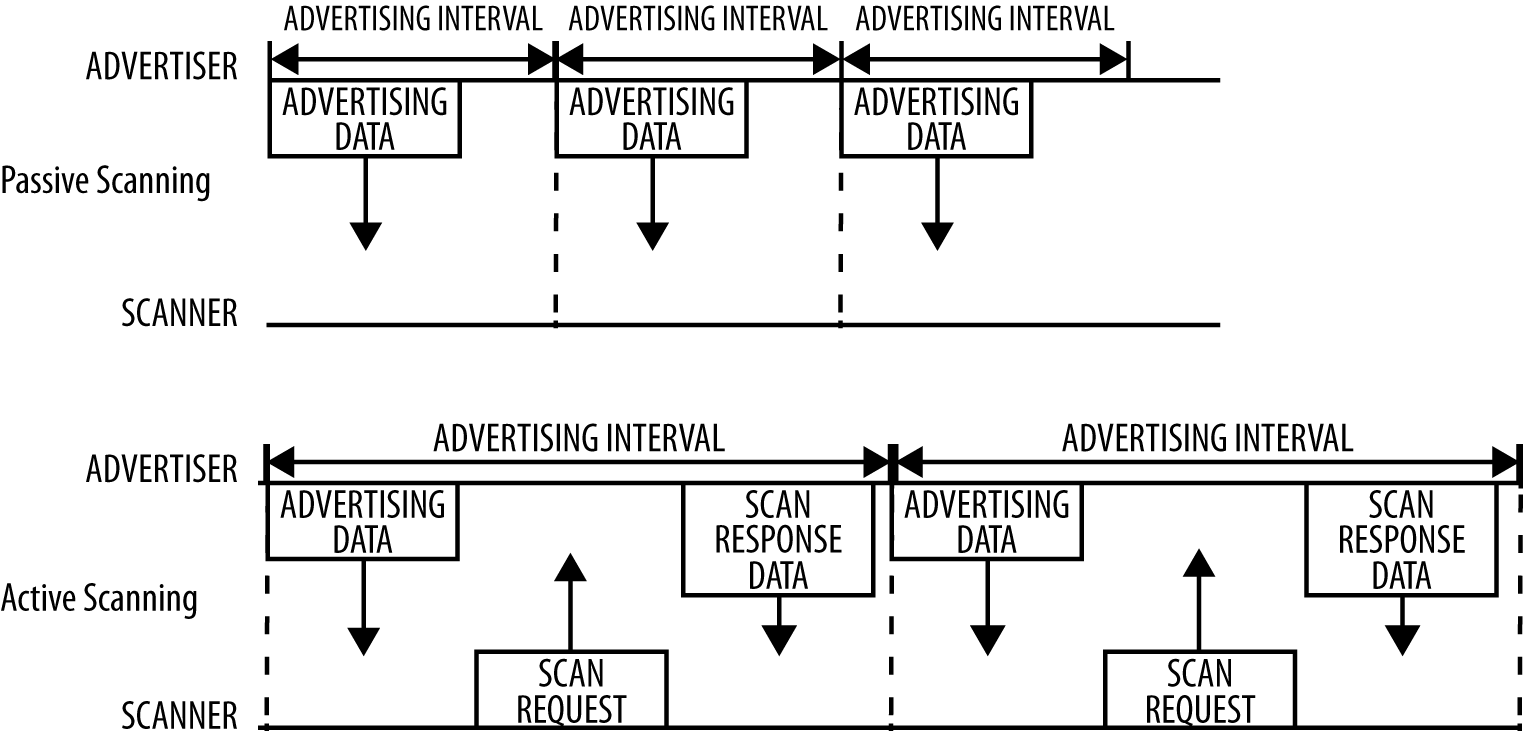
\includegraphics[scale=0.2]{images/advertising_scanning.png}
	\caption{Link Layer Advertising and Scanning}
\end{figure}
\paragraph{Link Layer Advertising Packet types}
\begin{figure}[ht]
	\centering
	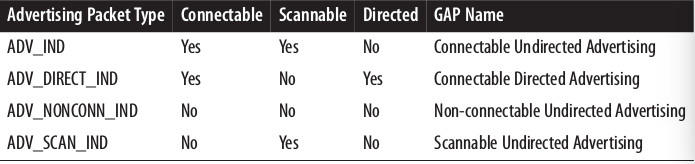
\includegraphics[scale=0.5]{images/advertising_packet_types.png}
	\caption{Link Layer Advertising Packet types}
\end{figure}
\paragraph{Link Layer Connections}
To establish a connection, a master first starts scanning to look for advertisers that are currently accepting connection requests. A connection is simply a sequence of data exchanges between the slave and the master at predefined times. Shown in Figure, each exchange is called \textbf{connection event}.
\begin{figure}[ht]
	\centering
	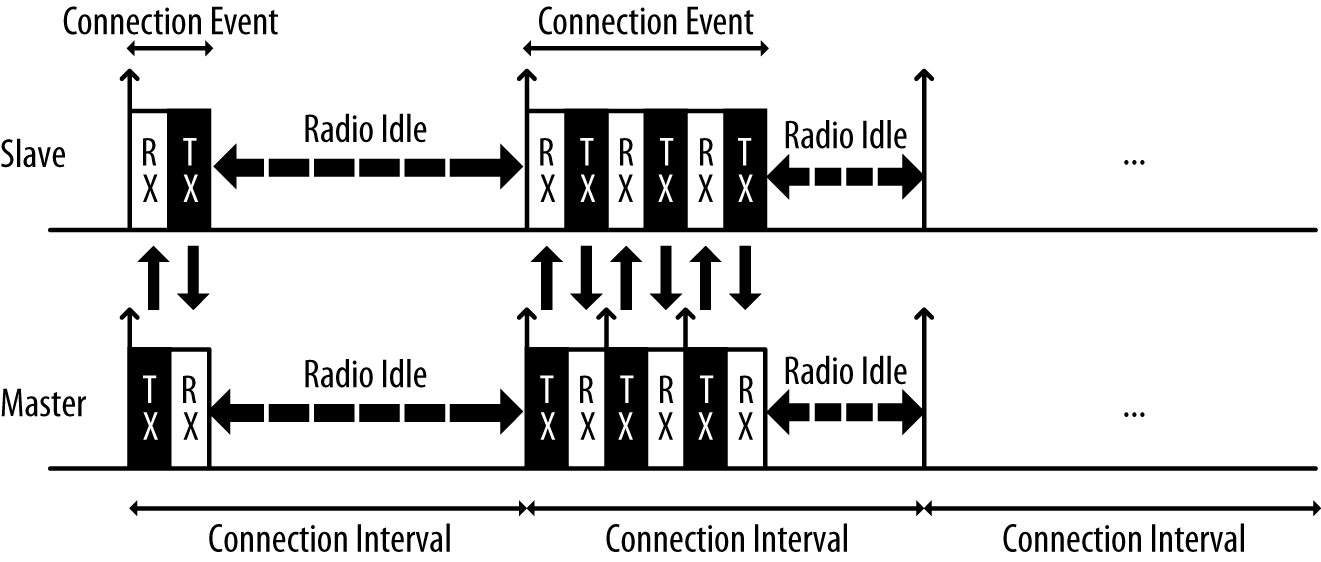
\includegraphics[scale=0.35]{images/connection_event.png}
	\caption{Link Layer connection event}
\end{figure}
\paragraph{Link Layer connection parameters}
\begin{enumerate}
	\item \textbf{Slave latency}: The number of connection events that a slave can choose to skip without risking a disconnection.
	\item \textbf{Connection interval}: The time between the beginnings of two consecutive connection events. This value ranges from 7.5 ms (high throughput) to 4s (lowest possible throughput but also least power hungry).
	\item \textbf{Connection supervision timeout}: The maximum time between two received valid data packets before a connection is considered lost.
\end{enumerate}
\subsection{The Host Layer}
This layer contains many of the protocols and profiles of BLE stack that are essential to the functioning of the upper layers of BLE. Some of these are:
\begin{itemize}
	\item L2CAP
	\item SMP
	\item GAP
	\item ATT
	\item GATT
\end{itemize}
\subsubsection{L2CAP}
\textbf{Logical Link Control and Adaptation Protocol} provides two main pieces of functionality:
\begin{enumerate}
	\item It serves as a \textbf{protocol multiplexer} that takes multiple protocols from the upper layers and encapsulated them into the standard BLE packet format (and vice versa).
	\item It also performs \textbf{fragmentation and recombination}, a process by which it takes large packets from the upper layers and breaks them up into chunks that fit into the 27-byte maximum payload size of the BLE packets on the transmit side. On the reception path, it receives multiple packets that have been fragmented and recombines them into a single large packet that will then be sent upstream to the appropriate entity in the upper layers of the host.
\end{enumerate}
\subsubsection{ATT}
\textbf{The Attribute Protocol} (ATT) is a simple client/server stateless protocol based on attributes presented by a device. In BLE, each device is a client, a server, or both, irrespective of whether it is a master of slave. A client requests data from a server, and a server sends data to clients. Each server contains data organized in the form of attributes each of which is assigned a \textbf{16-but attribute handle}, a \textbf{universally unique identifier} (UUID), a \textbf{set of permissions}, and finally of course, a \textbf{value}. The attribute handle is simply an identifier used to access an attribute value. The UUID specifies the type and nature of the data contained in the value. \\
The client and server perform various operations under this protocol such as searching for attributes, reading the values of attributes, writing values to attributes, etc. All of these operations are allowed based on the attribute permissions.
\subsubsection{SM}
\textbf{The Security Manager} (SM) is both a protocol and a series of security algorithms designed to provide the Bluetooth protocol stack with the ability to generate and exchange security keys, which then allow the peers to communicate securely over an encrypted link, to trust the identity of the remote device, and finally to hide the public Bluetooth Address if required to avoid malicious peers tracking a particular device.\\
The defined two roles, \textbf{Initiator} (always corresponds to the link layer master and therefor the GAP central) and \textbf{Responder} (link layer slave and hence the GAP peripheral).
\paragraph{SM Security Procedures}
The Security Manager provides support for the following three procedures:
\begin{enumerate}
	\item \textbf{Pairing}: Exchanging of the temporary key generated by the devices. This is done using algorithms like \textit{Just works, Passkey display, and Out of Band.}
	\item \textbf{Bonding}: Saving the key shared during pairing for future connections.
	\item \textbf{Encryption re-establishment}: Using the key stored during bonding to re-establish the connection.
\end{enumerate}
\paragraph{SM Security Mechanisms}
The SM specifies the following three types of security mechanisms that can be used to enforce various levels of security while in a connection or during the advertising procedure:
\begin{enumerate}
	\item \textbf{Encryption}: This mechanism consists of the full encryption of all packets transmitted over an established connection.
	\item \textbf{Privacy}: The privacy feature allows an advertiser to hide its public Bluetooth address by using temporary, randomly generated addresses that can be recognized by a scanner that is bonded with advertising device.
	\item \textbf{Signing}: With this mechanism, a device can send and unencrypted packet over an established connection that is digitally signed i.e. the source of which can be verified.
\end{enumerate}
\subsubsection{GAP}
\textbf{The Generic Access Profile} (GAP) dictates how devices interact with each other at a lower level, outside of the actual protocol stack, GAP can be considered to define the BLE topmost control layer, given that it specifies how devices perform control procedures such as devices discovery, connection, security establishment, and other to ensure interoperability and to allow data exchange to take place between devices from different vendors.
\paragraph{GAP Roles}
\begin{itemize}
	\item \textbf{Broadcaster}: Sends advertising packets for the purpose of broadcasting data.
	\item \textbf{Observer}: Scans for any broadcasted advertising packets in its range.
	\item \textbf{Central}: Scans for any advertising packet that is inviting a connection with a peripheral.
	\item \textbf{Peripheral}: Sends advertising packets for the purpose of connecting with a central.
\end{itemize}
There is no restriction on the number of centrals connected to the number of peripherals and vice-versa. 
\paragraph{GAP Modes and Procedures}
\begin{itemize}
	\item \textbf{Broadcast mode} (broadcaster device)
	\item \textbf{Observation procedure} (by observer device)
	\item \textbf{Discoverability mode} (Peripheral)
		\begin{enumerate} 
			\item Non discoverable
			\item Limited (discoverable only for a given time)
			\item General (discoverable and willing to connect with a central)
		\end{enumerate}
	\item \textbf{Discovery procedure} (by central)
		\begin{enumerate}
			\item Limiter discovery procedure (looks for and connects to peripherals with limited discoverable mode)
			\item General discovery procedure (looks for all peripherals and connects to them)
		\end{enumerate}
	\item \textbf{Connection establishment modes} (peripheral)
		\begin{enumerate}
			\item Non-connectable mode (Advertise only for the purpose of broadcasting)
			\item Directed connectable (Advertise to connect to a specific central)
			\item Undirected connectable (Advertise to connect to any central)
		\end{enumerate}
	\item \textbf{Connection establishment procedures} (by central)
		\begin{enumerate}
			\item  Auto connection (Uses white lists and connects to first advertising device that also happens to be on the list)
			\item General connection (Looks for all advertising device and then decides for each device if connection is to be made or not)
			\item Selective connection (Same as general connection procedure but with the use of white lists)
			\item Direct Connection (Look only for specific peripheral and if that peripheral happens to be advertising then connect to it)
		\end{enumerate}
	\item \textbf{Name Discovery Procedure}: Get name of the connected device via GATT transaction
	\item \textbf{Connection Parameters Update Procedure}: Can be requested by peripheral and/or imposed by the central.
	\item \textbf{Terminate Connection Procedure}: Connection is terminated and the reason message is given to the connected device.
\end{itemize}
\subsubsection{GATT}
\textbf{The Generic Attribute Profile} builds on the Attribute Protocol and adds a hierarchy and data abstraction model on top of it. This abstraction is described by the following figure:
\begin{figure}[ht]
	\centering
	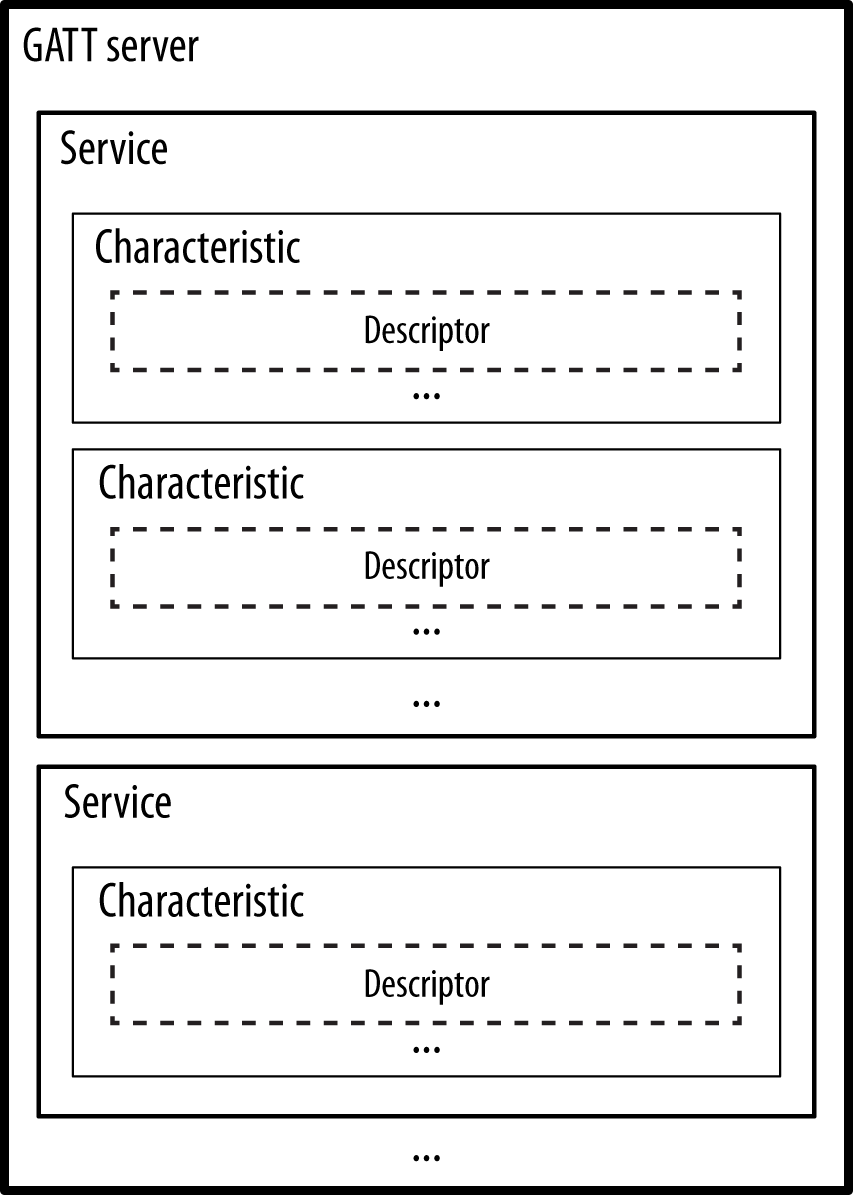
\includegraphics[scale=0.2]{images/gatt_server.png}
	\caption{GATT server}
\end{figure}
\paragraph{Attributes in GATT}
An attribute can be seen as the basic unit of data in a GATT server. An attribute contains the following fields of data:
\begin{enumerate}
	\item \textbf{Handle} (2 bytes)
	\item \textbf{UUID} (16, 4, 2 bytes)
	\item \textbf{Permissions} (R, W, RW, None)
	\item \textbf{Value} (up to 512 bytes)
\end{enumerate}
\paragraph{GATT operations}
\begin{itemize}
	\item \textbf{Exchange MTU} (Agreeing upon the maximum unit of transmission)
	\item \textbf{Discovery} (client finding the services at the server)
		\begin{enumerate}
			\item Service Discovery
			\item Characteristic Discovery
		\end{enumerate}
	\item \textbf{Reading Characteristics and Descriptors} (client collects information about the characteristics of various services)
	\item \textbf{Writing Characteristics and Descriptors} (client accesses and then attempts to change value of the characteristic values). The following two things are to be considered here are:
		\begin{enumerate}
			\item Insufficient Authentication (Key not available OR key send with Just Works)
			\item Insufficient Encryption (LTK available but link is not encrypted with it)
		\end{enumerate}
	\item \textbf{Server Initiated Updates} (Send asynchronously by the server whenever the value of any characteristic has been updated)
		\begin{enumerate}
			\item Characteristic Value Notification
			\item Characteristic Value Indication
		\end{enumerate}
\end{itemize}
\section{Assumptions and Dependencies}
In order for this project i.e. device driver for BlueNRG to work, the following dependencies are assumed:
\begin{itemize}
	\item A SoC system running on \textbf{Linux}.
	\item A SoC system having \textbf{SPI} support.
	\item \textbf{Bluez} on the system for testing and command line interaction.
	\item \textbf{BlueNRG} to be connected and used with the system via SPI.
\end{itemize}
The above mentioned dependencies are discussed in depth in the coming sections and chapters.
\section{Bluez The official Linux Bluetooth stack}
\textbf{BlueZ} is the official Linux Bluetooth protocol stack. It is an Open Source project distributed under the GNU General Public License (GPL). BlueZ kernel is part of the official Linux kernel since version 2.4.6.
\begin{figure}[ht]
	\centering
	
\includegraphics[width=3.5in, height=3in]{images/bluez_intro.png}
	\caption{Bluez the official Bluetooth stack of Linux}
\end{figure}
\subsection{History}
The Bluetooth technology was announced in May 1998 with the goal to create an easy usable cable replacement. But Bluetooth has proven to be more than a simple cable replacement technology with an enormous scope of applications and a rich set of standard protocol suite. The first steps into supporting Bluetooth with Linux were done by Axis Communications with their OpenBT Bluetooth Stack in April 1999. Also IBM released its BlueDrekar which was only available as binary modules. The problem of both stacks was that they are character driven, but the Bluetooth technology is for connecting devices. So it is better to integrate it into the Linux network layer and to use the socket interface as primary API.\\
On May 3, 2001, the Bluetooth protocol stack called BlueZ which was written by Qualcomm was released under GPL. The new stack followed the socket based approach. A socket in network programming represents the endpoint of a communication link. The idea is that from a software application's point of view, all data being passed through the link must go into or come out of the socket. Later it was picked up by Linus Torvalds and integrated into the Linux 2.4.6-pre2 kernel. This led to the Open Source community to support BlueZ as official Bluetooth Protocol Stack for Linux.
\subsection{The Bluetooth Stack}
The Bluetooth Stack is divided into three components.
\begin{enumerate}
	\item The controller
	\item The Host
	\item The Application
\end{enumerate}
Another important component is the Host Controller Interface.
\begin{figure}[ht]
	\centering
	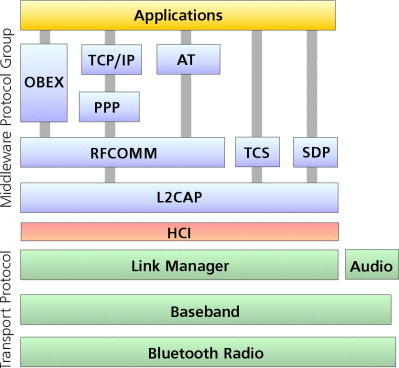
\includegraphics[scale=0.5]{images/bluetooth_stack.png}
	\caption{The Bluez Stack}
\end{figure}
The whole Bluetooth Stack has been divided into two component stacks in Linux. One portion of the stack is made part of the kernel space. The other portion is available as a separate toolkit for the users in the user-space.
\begin{figure}[ht]
	\centering
	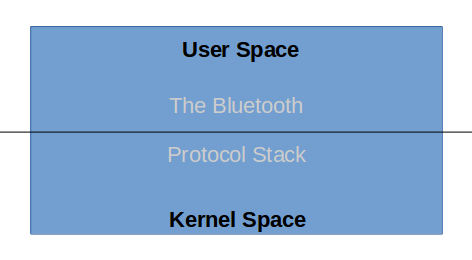
\includegraphics[width=3.5in, height=3in]{images/kernel_userspace.png}
	\caption{Stack division}
\end{figure}
The source for all of the kernel side code can be located in the Linux kernel at: \textbf{/net/Bluetooth}.\\
The Kernel side of the stack contains:
\begin{itemize}
	\item Low level protocols (L2CAP, RFCOMM, BNEP, HIDP, etc)
	\item Security (SSP, SMP)
	\item Hardware drivers
	\item Provides socket based interfaces to user space
	\begin{itemize}
		\item For data (L2CAP, RFCOMM, SCO, HCI)
		\item For control (MGMT, HCI, BNEP, HIDP)
	\end{itemize}
\end{itemize}
The source for the user-space side of Blue can be ne obtained from \textbf{http://www.bluez.org/download/}. It consists of the following things:
\begin{itemize}
	\item Bluetoothd
	\begin{itemize}
		\item Central daemon
		\item D-Bus interfaces for UI and other subsystems
		\item Reduces exposure to low details
		\item Extendible with plugins (eg neard for NFC)
	\end{itemize}
	\item Obexd
	\begin{itemize}
		\item Daemon for OBEX profiles
		\item D-Bus interface for UI
		\item Similar architecture to bluetoothd
	\end{itemize}
	\item Tools
	\begin{itemize}	
		\item Bluetoothctl – command line agent
		\item Btmon -HCI tracer
		\item Set of command line tools useful for testing, development and tracing
	\end{itemize}
\end{itemize}
The whole Bluez architecture is summed up by the following figure:
\begin{figure}[ht]
	\centering
	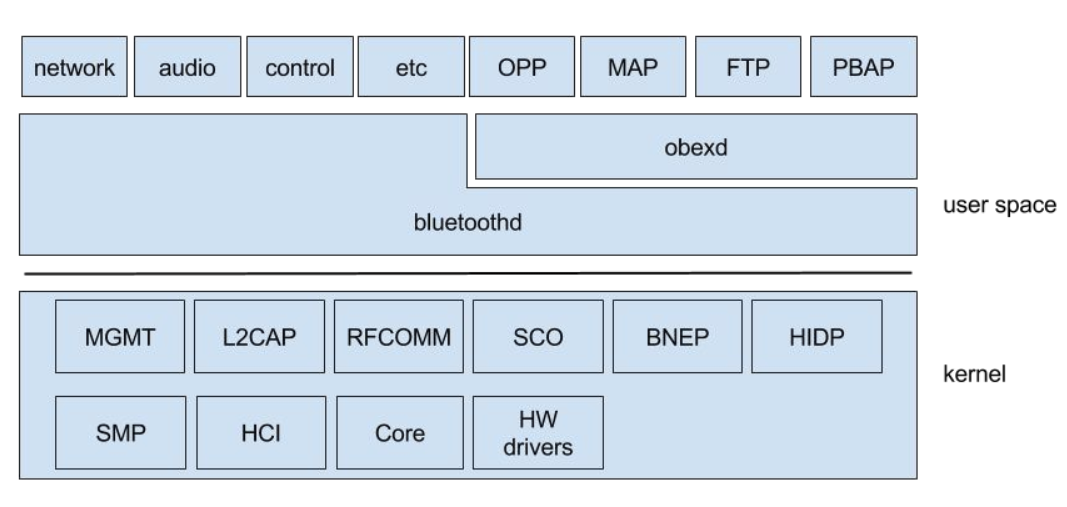
\includegraphics[width=3.5in, height=3in]{images/whole_bluez.png}
	\caption{The whole Bluez Stack}
\end{figure}
\section{BlueNRG}
The BlueNRG is a very low power Bluetooth Low Energy (BLE) single-mode network processor, compliant with Bluetooth specification v4.0. The BlueNRG can act as slave. The Bluetooth Low Energy stack runs on the embedded ARM Cortex-M0 core. The stack is stored on the on-chip non-volatile Flash memory and can be easily upgraded via SPI. The device comes pre-programmed with a production-ready stack image (whose version could change at any time without notice). A different or more up-to-date stack image can be downloaded from the ST web site and programmed on the device through the ST provided software tools. The BlueNRG allows applications to meet the tight advisable peak current requirements imposed by the use of standard coin cell batteries. The maximum peak current is only 10 mA at 1 dBm of output power. Ultra low-power sleep modes and very short transition times between operating modes allow very low average current consumption, resulting in longer battery life. The BlueNRG offers the option of interfacing with external microcontrollers using SPI transport layer.
\subsection{General Description}
The BlueNRG is a single-mode Bluetooth low energy slave network processor, compliant with the Bluetooth specification v4.0.\\
It integrates a 2.4 GHz RF transceiver and a powerful Cortex-M0 microcontroller, on which a complete power-optimized stack for Bluetooth single mode protocol runs, providing:
\begin{itemize}
	\item Slave role support
	\item GAP: peripheral, broadcaster roles
	\item ATT/GATT: client and server
	\item SM: privacy, authentication and authorization
	\item L2CAP
	\item Link Layer: AES-128 encryption and decryption
\end{itemize}
An on-chip non-volatile Flash memory allows on-field Bluetooth low energy stack upgrade.\\
The device allows applications to meet the tight advisable peak current requirements imposed by the use of standard coin cell batteries. If the high efficiency embedded DC-DC step-down converter is used, the maximum input current is only 15 mA at the highest output power (+8 dBm). Even if the DC-DC converter is not used, the maximum input current is only 29 mA at the highest output power, still preserving battery life.\\
Ultra low-power sleep modes and very short transition time between operating modes result in very low average current consumption during real operating conditions, providing very long battery life.\\
Two different external matching networks are suggested: standard mode (TX output power up to +5 dBm) and high power mode (TX output power up to +8 dBm).\\
The external host application processor, where the application resides, is interfaced with the BlueNRG through an application controller interface protocol based on a standard SPI interface.
\begin{figure}[ht]
	\centering
	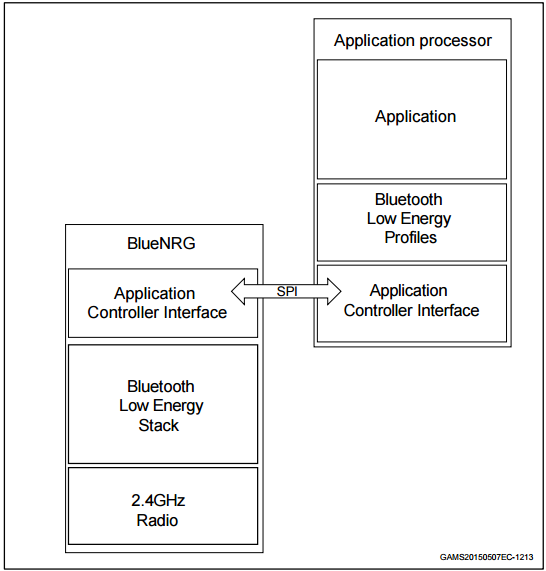
\includegraphics[width=3.5in, height=3in]{images/bluenrg_spi.png}
	\caption{BlueNRG SPI Interface}
\end{figure}
\subsection{Pin Description}
\begin{table}[ht]
	\centering
	\scalebox{0.5}{
	\begin{tabular}{|K{5cm} | K{5cm} | K{3cm} | K{2cm} | K{10cm}|}
		\toprule
		\rowcolor{Gray}
		\textbf{QFN32 pins} & \textbf{WLCSP pins}  & \textbf{Name} & \textbf{I/O} & \textbf{Description} \\
		\hline
		1 & E2 & SPI\_MOSI & I & SPI\_MOSI \\
		\hline
		2 & E1 & SPI\_CLK & I & SPI\_CLK \\
		\hline
		3 & D2 & SPI\_IRQ & O & SPI\_IRQ \\
		\hline
		4 & D1 & TEST1 & IO & Test pin \\
		\hline
		5 & C1 & VBAT3 & VDD & 2.0-3.6 battery voltage input \\
		\hline
		6 & C2 & TEST2 & IO & Test pin connected GND \\
		\hline
		7 & B1 & TEST3 & IO & Test pin connected GND \\
		\hline
		8 & B2 & TEST4 & IO & Test pin connected GND\\
		\hline
		9 & A1 & TEST5 & IO & Test pin connected GND\\
		\hline
		10 & B3 & TEST6 & IO & Test pin connected GND\\
		\hline
		11 & A2 & TEST7 & IO & Test pin connected GND\\
		\hline
		12 & A3 & VDD1V8 & O & 1.8 V digital core\\
		\hline
		13 & A4 & TEST8 & IO & Test pin not connected\\
		\hline
		14 & A5 & TEST9 & IO & Test pin not connected\\
		\hline
		15 & B4 & TEST11 & IO & Test pin not connected (QFN32), Test pin connected to GND (WLCSP)\\ 
		\hline
		16 & B5 & TEST12 & IO & Test pin not connected (QFN32), Test pin connected to GND (WLCSP) \\
		\hline
		17 & A6 & FXTAL1 & I & 16/32 MHz crystal\\
		\hline
		18 & B6 & FCTAL0 & I & 16/32 MHz crystal\\
	\bottomrule
	\end{tabular}}
	\caption{BlueNRG Pin Description part-I}
\end{table}
\begin{table}[ht]
	\centering
	\scalebox{0.5}{
	\begin{tabular}{|K{5cm} | K{5cm} | K{3cm} | K{2cm} | K{10cm}|}
		\toprule
		\rowcolor{Gray}
		\textbf{QFN32 pins} & \textbf{WLCSP pins}  & \textbf{Name} & \textbf{I/O} & \textbf{Description} \\
		19 & - & VBAT2 & VDD & 2.0-3.6 nattery voltage input\\
		\hline
		20 & C6 & RF1 & IO & Antenna + matching circuit\\
		\hline
		21 & D6 & RF0 & IO & Antenna + matching circuit\\
		\hline
		22 & E6 & SXTAL1 & I & 32 KHz crystal\\
		\hline
		23 & E5 & SXTAL0 & I & 32 KHz crystal\\
		\hline
		24 & D5 & VBAT1 & VDD & 2.0-3.6 battery voltage input\\
		\hline
		25 & E4 & RESETN & I & Reset\\
		\hline
		26 & F6 & SMPSFILT1 & O &  SMPS output\\
		\hline
		27 & - & NO\_SMPS & I & Power management strategy selection\\
		\hline
		28 & F5 & SMPSFILT2 & IO & SMPS input-ouput\\
		\hline
		29 & F3 & VDD1V2 & O & 1.2 V digital core\\
		\hline
		30 & E3 & TEST10 & IO & TEST pin connected to GND\\
		\hline
		31 & F2 & SPI\_CS & I & SPI\_CS\\
		\hline
		32 & F1 & SPI\_MISO & O & SPI\_MISO\\
		\hline
		- & C3 & GND & GND & Ground\\
		\hline
		- & D3 & GND & GND & Ground\\
		\hline
		- & D4 & GND & GND & Ground\\
		\hline
		- & F4 & SMPS-GND & GND & SMPS ground\\
	\bottomrule
	\end{tabular}}
	\caption{BlueNRG Pin Description part-II}
\end{table}
\subsection{Core, Memory and Peripherals}
The device contains an ARM Cortex-M0 microcontroller core that supports ultra-low leakage state retention mode and almost instantaneously returning to fully active mode on critical events. \\
The memory subsystem consists of 64 KB Flash, and 12 KB RAM , divided in two blocks of 6 KB (RAM1 and RAM2). Flash is used for the M0 program. No RAM or FLASH resources are available to the external microcontroller driving the BlueNRG.\\
The application controller interface (ACI) uses a standard SPI slave interface as transport layer, basing in five physical wires:
\begin{itemize}
	\item 2 control wires (clock and slave select) 
	\item 2 data wires with serial shift-out (MOSI and MISO) in full duplex 
	\item 1 wire to indicate data availability from the slave
\end{itemize}
\begin{table}[ht]
	\centering
	\scalebox{0.8}{
		\begin{tabular}{|c|c|c|c|}
			\toprule
			\rowcolor{Gray}
			\textbf{Name} & \textbf{Direction} &\textbf{Width} &\textbf{Description} \\
			\hline
			SPI\_CS & In & 1 & SPI slave select = SPI enable\\
			\hline
			SPI\_CCL & In & 1 & SPI clock (max 8MHz)\\
			\hline
			SPI\_MOSI & In & 1 & Master output, slave input\\
			\hline
			SPI\_MISO & Out & 1 & Master input, slave output\\
			\hline
			SPI\_IRQ & Out & 1 & Slave has data for master\\
			\bottomrule
		\end{tabular}
	}
	\caption{SPI Description}
\end{table}
All the SPI pins have an internal pull-down except for the CSN that has a pull-up. All the SPI pins, except the CSN, are in high impedance state during the low-power states. The IRQ pin needs a pull-down external resistor.
\subsection{Power Management}
The device integrates both a low dropout voltage regulator (LDO) and a step-down DC-DC converter, and one of them can be used to power the internal circuitry. However even when the LDO is used, the stringent maximum current requirements, which are advisable when coin cell batteries are used, can be met and further improvements can be obtained with the DC-DC converter at the sole additional cost of an inductor and a capacitor.
\subsection{Bluetooth Low Energy Radio}
The device integrates an RF transceiver compliant with the Bluetooth specification and the standard national regulations in the unlicensed 2.4 GHz ISM band. The RF transceiver requires very few external discrete components. It provides 96 dB link budgets with excellent link reliability, keeping the maximum peak current below 15 mA. In Transmit mode, the power amplifier (PA) drives the signal generated by the frequency synthesizer out to the antenna terminal through a very simple external network. The power delivered as well as the harmonic content depends on the external impedance seen by the PA.
\subsection{Operating Modes}
Several operating modes are defined for the BlueNRG:
\begin{itemize}
	\item Reset mode
	\item Sleep mode 
	\item Standby mode 
	\item Active mode 
	\item Radio mode 
	\begin{itemize}
		\item Receive Radio mode 
		\item Transmit Radio mode
	\end{itemize}
\end{itemize}
In Reset mode, the device is in ultra-low power consumption: all voltage regulators, clocks and the RF interface are not powered. The device enters Reset mode by asserting the external reset signal. As soon as it is de-asserted, the device follows the normal activation sequence to transit to Active mode. \\
In Sleep mode either the low speed crystal oscillator or the low speed ring oscillator are running, whereas the high speed oscillators are powered down as well as the RF interface. The state of the device is retained and the content of the RAM is preserved. Depending on the application, part of the RAM (RAM2 block) can be switched off during sleep to save more power (refer to stack mode 1, described in UM1868). \\
While in Sleep mode, the device waits until an internal timer expires and then it goes into Active mode. The transition from Sleep mode to Active mode can also be activated through the SPI interface. \\
Standby mode and Sleep mode are equivalent but the low speed frequency oscillators are powered down. In Standby mode the device can be activated through the SPI interface. \\
In Active mode the device is fully operational: all interfaces, including SPI and RF, are active as well as all internal power supplies together with the high speed frequency oscillator. The MCU core is also running. \\
Radio mode differs from Active mode as also the RF transceiver is active and it is capable of either transmitting or receiving.
\begin{figure}[ht]
	\centering
	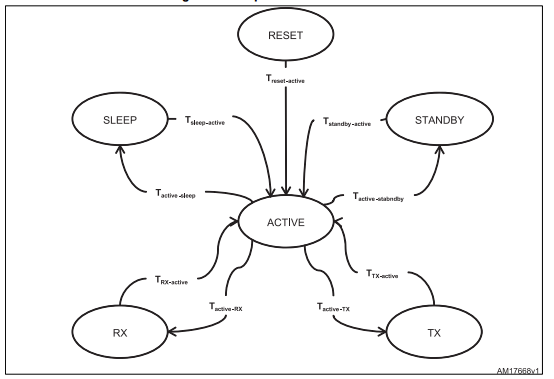
\includegraphics[width=3.5in, height=3in]{images/operating_modes.png}
	\caption{BlueNRG Operating Modes}
\end{figure}
\begin{table}[ht]
	\centering
	\scalebox{0.7}{
		\begin{tabular}{|K{2cm}| K{4cm} | K{2cm}|K{2cm}|K{2cm}|K{2cm}|K{2cm}|K{2cm}|K{2cm}|}
			\toprule
			\rowcolor{Gray}
			\textbf{State} & \textbf{Digital LDO} & \textbf{SPI} & \textbf{LSOSC} & \textbf{HSOSC} & \textbf{Core} & \textbf{RF synt.} & \textbf{RX chain} & \textbf{TX chain} \\
			\hline
			Reset & OFF Register contents lost & OFF & OFF & OFF & OFF & OFF & OFF & OFF \\
			\hline
			Standby & ON Register contents retained & ON & OFF & OFF & OFF & OFF & OFF & OFF \\
			\hline
			Sleep & ON Register contents retained & ON & ON & OFF & OFF & OFF & OFF & OFF \\
			\hline
			Active & ON Register contents retained & ON & . & ON & ON & OFF & OFF & OFF \\
			\hline
			RX & ON Register contents retained & ON & . & ON & ON & ON & ON & OFF \\
			\hline
			TX & ON Register contents retained & ON & . & ON & ON & ON & OFF & ON\\
			\bottomrule
		\end{tabular}
	}
	\caption{BlueNRG operating modes summary}
\end{table}
\section{Product Perspective}
BlueNRG is a network processor. This means it implement in it, the stack of both the host and the controller. But for the intent of this project, we are interested only in the controller stack of BlueNRG as the host part of the stack will be provided by a Linux host. As is defined in the specification a host and a controller must communicate using the HCI protocol. And Bluez is of course capable of providing this interface to our controller: BlueNRG. Since BlueNRG uses SPI as the transport layer, there is a need to write a SPI driver that can take HCI commands from Bluez stack and send them over to BlueNRG. The response to HCI commands is of course HCI events. These are communicated using the same channels i.e. SPI. \\
Once this host and controller setup is ready, it is time to communicate with another Bluetooth Low Energy complaint device. The communication between this other device and our host (the Linux machine) will happen through one of many Bluetooth Low Energy profiles in the application layer. The driver and BlueNRG need not concern itself with what these applications are. All it needs to care about is the HCI commands that is going to receive from the host over SPI and sending back appropriate responses for the send commands. This is possible because any operation that is needed to performed by the application will eventually be converted into a HCI command. All of this is taken care of by the Bluez stack between its user-space and then the kernel side components discussed earlier. \\
The follow of control or data is summarized in the following flow diagram.
\section{Flow Diagram}
\begin{figure}[ht]
	\centering
	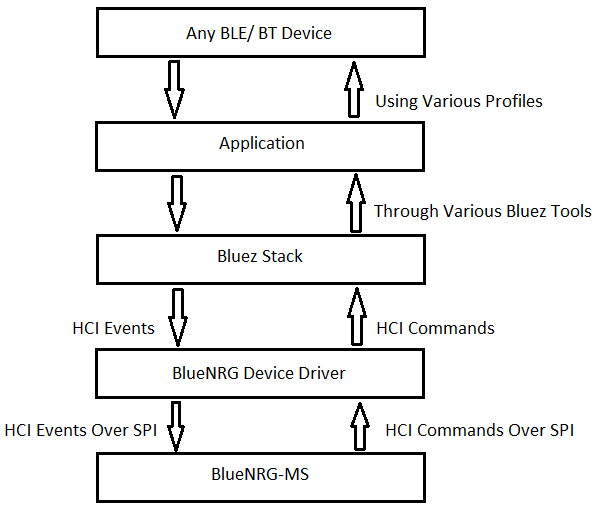
\includegraphics[scale=0.5]{images/flow_chart.png}
	\caption{Flow Chart}
\end{figure}
